\PassOptionsToPackage{unicode=true}{hyperref} % options for packages loaded elsewhere
\PassOptionsToPackage{hyphens}{url}
%
\documentclass[]{article}
\usepackage{lmodern}
\usepackage{amssymb,amsmath}
\usepackage{ifxetex,ifluatex}
\usepackage{fixltx2e} % provides \textsubscript
\ifnum 0\ifxetex 1\fi\ifluatex 1\fi=0 % if pdftex
  \usepackage[T1]{fontenc}
  \usepackage[utf8]{inputenc}
  \usepackage{textcomp} % provides euro and other symbols
\else % if luatex or xelatex
  \usepackage{unicode-math}
  \defaultfontfeatures{Ligatures=TeX,Scale=MatchLowercase}
\fi
% use upquote if available, for straight quotes in verbatim environments
\IfFileExists{upquote.sty}{\usepackage{upquote}}{}
% use microtype if available
\IfFileExists{microtype.sty}{%
\usepackage[]{microtype}
\UseMicrotypeSet[protrusion]{basicmath} % disable protrusion for tt fonts
}{}
\IfFileExists{parskip.sty}{%
\usepackage{parskip}
}{% else
\setlength{\parindent}{0pt}
\setlength{\parskip}{6pt plus 2pt minus 1pt}
}
\usepackage{hyperref}
\hypersetup{
            pdftitle={Advanced Macro},
            pdfauthor={Hans Martinez},
            pdfborder={0 0 0},
            breaklinks=true}
\urlstyle{same}  % don't use monospace font for urls
\usepackage[margin=1in]{geometry}
\usepackage{color}
\usepackage{fancyvrb}
\newcommand{\VerbBar}{|}
\newcommand{\VERB}{\Verb[commandchars=\\\{\}]}
\DefineVerbatimEnvironment{Highlighting}{Verbatim}{commandchars=\\\{\}}
% Add ',fontsize=\small' for more characters per line
\usepackage{framed}
\definecolor{shadecolor}{RGB}{248,248,248}
\newenvironment{Shaded}{\begin{snugshade}}{\end{snugshade}}
\newcommand{\AlertTok}[1]{\textcolor[rgb]{0.94,0.16,0.16}{#1}}
\newcommand{\AnnotationTok}[1]{\textcolor[rgb]{0.56,0.35,0.01}{\textbf{\textit{#1}}}}
\newcommand{\AttributeTok}[1]{\textcolor[rgb]{0.77,0.63,0.00}{#1}}
\newcommand{\BaseNTok}[1]{\textcolor[rgb]{0.00,0.00,0.81}{#1}}
\newcommand{\BuiltInTok}[1]{#1}
\newcommand{\CharTok}[1]{\textcolor[rgb]{0.31,0.60,0.02}{#1}}
\newcommand{\CommentTok}[1]{\textcolor[rgb]{0.56,0.35,0.01}{\textit{#1}}}
\newcommand{\CommentVarTok}[1]{\textcolor[rgb]{0.56,0.35,0.01}{\textbf{\textit{#1}}}}
\newcommand{\ConstantTok}[1]{\textcolor[rgb]{0.00,0.00,0.00}{#1}}
\newcommand{\ControlFlowTok}[1]{\textcolor[rgb]{0.13,0.29,0.53}{\textbf{#1}}}
\newcommand{\DataTypeTok}[1]{\textcolor[rgb]{0.13,0.29,0.53}{#1}}
\newcommand{\DecValTok}[1]{\textcolor[rgb]{0.00,0.00,0.81}{#1}}
\newcommand{\DocumentationTok}[1]{\textcolor[rgb]{0.56,0.35,0.01}{\textbf{\textit{#1}}}}
\newcommand{\ErrorTok}[1]{\textcolor[rgb]{0.64,0.00,0.00}{\textbf{#1}}}
\newcommand{\ExtensionTok}[1]{#1}
\newcommand{\FloatTok}[1]{\textcolor[rgb]{0.00,0.00,0.81}{#1}}
\newcommand{\FunctionTok}[1]{\textcolor[rgb]{0.00,0.00,0.00}{#1}}
\newcommand{\ImportTok}[1]{#1}
\newcommand{\InformationTok}[1]{\textcolor[rgb]{0.56,0.35,0.01}{\textbf{\textit{#1}}}}
\newcommand{\KeywordTok}[1]{\textcolor[rgb]{0.13,0.29,0.53}{\textbf{#1}}}
\newcommand{\NormalTok}[1]{#1}
\newcommand{\OperatorTok}[1]{\textcolor[rgb]{0.81,0.36,0.00}{\textbf{#1}}}
\newcommand{\OtherTok}[1]{\textcolor[rgb]{0.56,0.35,0.01}{#1}}
\newcommand{\PreprocessorTok}[1]{\textcolor[rgb]{0.56,0.35,0.01}{\textit{#1}}}
\newcommand{\RegionMarkerTok}[1]{#1}
\newcommand{\SpecialCharTok}[1]{\textcolor[rgb]{0.00,0.00,0.00}{#1}}
\newcommand{\SpecialStringTok}[1]{\textcolor[rgb]{0.31,0.60,0.02}{#1}}
\newcommand{\StringTok}[1]{\textcolor[rgb]{0.31,0.60,0.02}{#1}}
\newcommand{\VariableTok}[1]{\textcolor[rgb]{0.00,0.00,0.00}{#1}}
\newcommand{\VerbatimStringTok}[1]{\textcolor[rgb]{0.31,0.60,0.02}{#1}}
\newcommand{\WarningTok}[1]{\textcolor[rgb]{0.56,0.35,0.01}{\textbf{\textit{#1}}}}
\usepackage{longtable,booktabs}
% Fix footnotes in tables (requires footnote package)
\IfFileExists{footnote.sty}{\usepackage{footnote}\makesavenoteenv{longtable}}{}
\usepackage{graphicx,grffile}
\makeatletter
\def\maxwidth{\ifdim\Gin@nat@width>\linewidth\linewidth\else\Gin@nat@width\fi}
\def\maxheight{\ifdim\Gin@nat@height>\textheight\textheight\else\Gin@nat@height\fi}
\makeatother
% Scale images if necessary, so that they will not overflow the page
% margins by default, and it is still possible to overwrite the defaults
% using explicit options in \includegraphics[width, height, ...]{}
\setkeys{Gin}{width=\maxwidth,height=\maxheight,keepaspectratio}
\setlength{\emergencystretch}{3em}  % prevent overfull lines
\providecommand{\tightlist}{%
  \setlength{\itemsep}{0pt}\setlength{\parskip}{0pt}}
\setcounter{secnumdepth}{0}
% Redefines (sub)paragraphs to behave more like sections
\ifx\paragraph\undefined\else
\let\oldparagraph\paragraph
\renewcommand{\paragraph}[1]{\oldparagraph{#1}\mbox{}}
\fi
\ifx\subparagraph\undefined\else
\let\oldsubparagraph\subparagraph
\renewcommand{\subparagraph}[1]{\oldsubparagraph{#1}\mbox{}}
\fi

% set default figure placement to htbp
\makeatletter
\def\fps@figure{htbp}
\makeatother

\usepackage{etoolbox}
\makeatletter
\providecommand{\subtitle}[1]{% add subtitle to \maketitle
  \apptocmd{\@title}{\par {\large #1 \par}}{}{}
}
\makeatother

\title{Advanced Macro}
\providecommand{\subtitle}[1]{}
\subtitle{Assignment 2}
\author{Hans Martinez}
\date{Oct 04, 2020}

\begin{document}
\maketitle

\hypertarget{competitive-equilibrium}{%
\subsection{Competitive equilibrium}\label{competitive-equilibrium}}

Arrow-Debreu competitive equilibrium consists of prices
\(\{p_t,w_t,r_t\}_{t=0}^{\infty}\), allocations for the firm
\(\{y_t,k_t^d,l_t^d\}_{t=0}^{\infty}\) and the allocations for household
\(\{c_t,k_t^s,l_t^s\}_{t=0}^{\infty}\) such that,

\begin{itemize}
\item
  Given a sequence of prices \(\{p_t,w_t,r_t\}_{t=0}^{\infty}\), the
  firm allocation \(\{y_t,k_t^d,l_t^d\}_{t=0}^{\infty}\) solves the firm
  problem, \begin{equation}
            \begin{split}
                \max_{\{y_t,k_t,l_t\}_{t=0}^{\infty}}&\sum_{t=0}^{\infty}
                p_t(y_t-r_tk_t-w_tl_t)\\
                \text{s.t.  }&y_t=zk_t^{\alpha}l_t^{1-\alpha}, \forall t\geq 0;\\
                &y_t,k_t,l_t\geq 0, \forall t \geq 0.
            \end{split}
            \end{equation}
\item
  Given a sequence of prices \(\{p_t,w_t,r_t\}_{t=0}^{\infty}\), the
  household allocation \(\{c_t,k_t^s,l_t^s\}_{t=0}^{\infty}\) solves the
  household problem, \begin{equation}
            \begin{split}
                \max_{\{c_t,k_{t+1},l_t\}_{t=0}^{\infty}}&\sum_{t=0}^{\infty}
                \beta ^t(\frac{c_t^{1-\sigma}}{1-\sigma}-\chi \frac{l_t^{1+\eta}}{1+\eta})\\
                \text{s.t.  }& \sum_{t=0}^{\infty}p_t(c_t+K_{t+1}-(1-\delta)k_t)
                \leq\sum_{t=0}^{\infty}p_t(r_tk_t+w_tl_t);\\
                &0\leq l_t\leq 1,0\leq k_t\leq k_0, c_t\geq 0, k_{t+1}\geq 0,\forall t \geq 0;\\
                &k_0 \text{ given.}
            \end{split}
            \end{equation}
\item
  The market clear conditions, \begin{equation*}
            \begin{split}
                zk_t^{\alpha}l_t^{1-\alpha}+(1-\delta)k_t&=c_t+k_{t+1} ;\\
                l_t^d&=l_t^s    ;\\
                k_t^d&=k_t^s    .
            \end{split}
            \end{equation*}
\end{itemize}

\hypertarget{steady-state}{%
\subsection{Steady state}\label{steady-state}}

For firm problem, \begin{equation}
            \begin{split}
                r_t =&z\alpha k_t^{\alpha -1}l_t^{1-\alpha}\\
                w_t =&z(1-\alpha) k_t^{\alpha}l_t^{-\alpha}\\
                r_tk_t+w_tl_t&=zk_t^{\alpha}l_t^{1-\alpha}
            \end{split}
            \end{equation}

Then for household problem, \begin{equation}
            \begin{split}
                \mathcal{L}(\{c_t,k_{t+1},l_t\}_{t=0}^{\infty};\lambda_t)=&\sum_{t=0}^{\infty}
                \beta ^t(\frac{c_t^{1-\sigma}}{1-\sigma}-\chi \frac{l_t^{1+\eta}}{1+\eta})+\lambda_t(\sum_{t=0}^{\infty}p_t(zk_t^{\alpha}l_t^{1-\alpha}-c_t-k_{t+1}+(1-\delta)k_t)\\
                \frac{\partial \mathcal{L}}{\partial c_t}=&\beta^tc_t^{-\sigma}-\lambda_t p_t=0,\\
                \frac{\partial \mathcal{L}}{\partial l_t}=&-\beta^t\chi l_t^{\eta}+\lambda_t p_tz(1-\alpha) k_t^{\alpha}l_t^{-\alpha}=0,\\
                \frac{\partial \mathcal{L}}{\partial k_t}=&\lambda_t p_t(z\alpha k_t^{\alpha -1}l_t^{1-\alpha}+1-\delta)-\lambda_{t-1}p_{t-1}=0,\\
                c_t=&zk_t^{\alpha}l_t^{1-\alpha}-k_{t+1}+(1-\delta)k_t
            \end{split}
            \end{equation}

For Steady state, \(p_0=1\), then, \begin{equation}\label{ssfoc}
            \begin{split}
                &c^{\sigma} l^{\eta}=
                z(1-\alpha)k^{\alpha}l^{-\alpha}/\chi\\
                &z\alpha k^{\alpha -1}l^{1-\alpha}=
                1/\beta -1 +\delta\\
                &c=zk^{\alpha}l^{1-\alpha}-\delta k
            \end{split}
            \end{equation}\\
\begin{equation*}
                M=\frac{k}{l}=\left(\frac{z\alpha \beta}{1-\beta +\beta \delta}\right)^{\frac{1}{1-\alpha}},
            \end{equation*} \begin{equation*}
                N=\frac{c}{l}=z(\frac{k}{l})^{\alpha}-\delta \frac{k}{l}=zM^{\alpha}-\delta M,
            \end{equation*} \begin{equation*}
            \begin{split}
                (lN)^{\sigma}l^{\eta}=&
                z(1-\alpha)(\frac{k}{l})^{\alpha}/\chi\Rightarrow\\
                l^{\sigma+\eta}&=\frac{z(1-\alpha)M^{\alpha}}{\chi N^{\sigma}} \Rightarrow\\
                l_{ss}=&\left(\frac{z(1-\alpha)M^{\alpha}}{\chi N^{\sigma}}\right)^{\frac{1}{\sigma+\eta}},
            \end{split}
            \end{equation*}

Then, \begin{equation*}
            \begin{split}
                k_{ss}=&Ml\\
                c_{ss}=&Nl\\
                y_{ss}=&zk^{\alpha}l^{1-\alpha}=zM^{\alpha}l\\
                r_{ss}=&\alpha zk^{\alpha-1}l^{1-\alpha}=\alpha zM^{\alpha -1}\\
                w_{ss}=&(1-\alpha)zk^{\alpha}l^{\alpha}=(1-\alpha)zM^{\alpha}.
            \end{split}
            \end{equation*}

\hypertarget{social-planner-problem}{%
\subsection{Social planner problem}\label{social-planner-problem}}

The problem of the social planner is that, given the initial capital
\(k_0\), \begin{equation}\label{SPP1}
                \begin{split}
                    w( k_0)&=\max_{\{c_t, k_t, l_t \}_{t=0}^{\infty}}
                    \sum_{t=0}^{\infty}
                    \beta ^t(\frac{c_t^{1-\sigma}}{1-\sigma}-\chi \frac{l_t^{1+\eta}}{1+\eta})\\
                    s.t. \;\;zk_t^{\alpha}l_t^{1-\alpha}&=c_t+k_{t+1}-(1-\delta)k_t, \;\;\forall t\geq 0\\
                    c_t&\geq0,\;k_t\geq0,\;0\leq l_t\leq 1,  \;\;\forall t\geq 0\\
                    k_0&\text{ is given.}
                \end{split}
            \end{equation}

Bellman equation, \begin{equation}
                V(k)=\max_{\begin{smallmatrix}0\leq l\leq 1
                    \\0\leq k'\leq zk^{\alpha}l^{1-\alpha}+(1-\delta)k\end{smallmatrix}}
                    \{\frac{(zk^{\alpha}l^{1-\alpha}+(1-\delta)k-k')^{1-\sigma}}{1-\sigma}-\chi \frac{l^{1+\eta}}{1+\eta}+\beta \mathbb{E}V(k')\}
            \end{equation}

\hypertarget{vfi}{%
\subsection{VFI}\label{vfi}}

\href{https://github.com/hans-mtz/AdvMacro/blob/master/A2.jl}{Julia
code: click here.}

\begin{Shaded}
\begin{Highlighting}[]
\CommentTok{# Julia code}
\CommentTok{# See A2.jl}
\end{Highlighting}
\end{Shaded}

\begin{figure}

{\centering 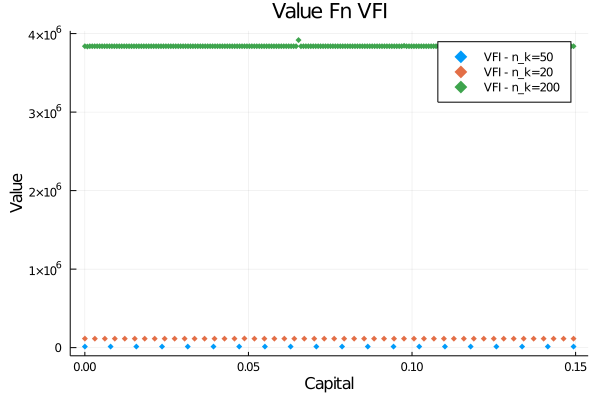
\includegraphics[width=0.65\linewidth]{Assignment2/graphs/VFI_V} 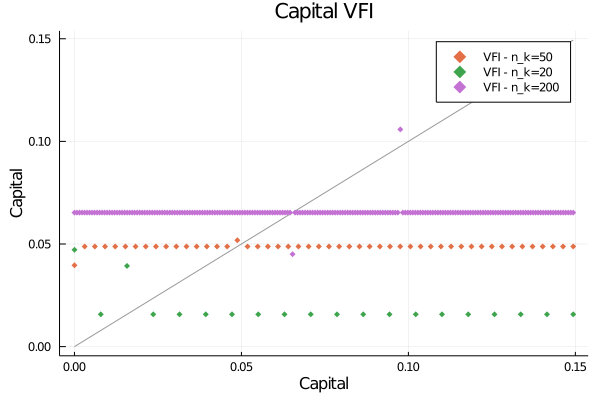
\includegraphics[width=0.65\linewidth]{Assignment2/graphs/VFI_cap} 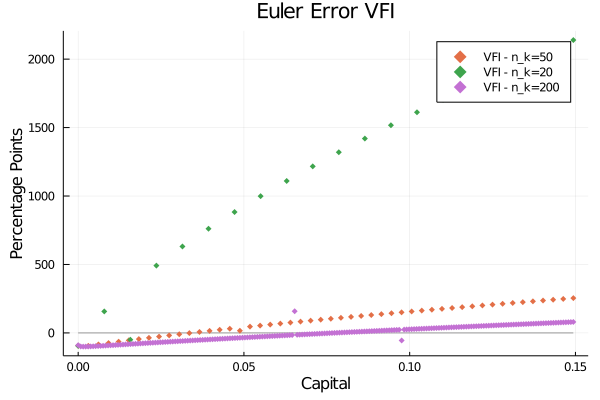
\includegraphics[width=0.65\linewidth]{Assignment2/graphs/VFI_Euler} 

}

\caption{Plain VFI}\label{fig:unnamed-chunk-2}
\end{figure}

\begin{figure}

{\centering 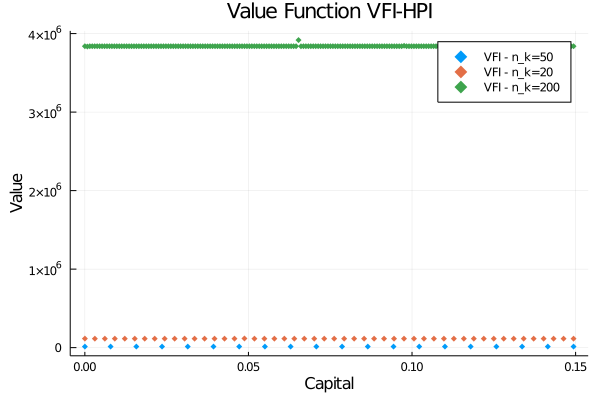
\includegraphics[width=0.65\linewidth]{Assignment2/graphs/HPI_V} 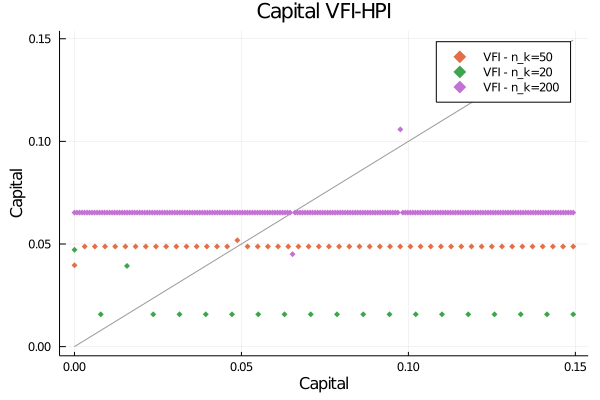
\includegraphics[width=0.65\linewidth]{Assignment2/graphs/HPI_Cap} 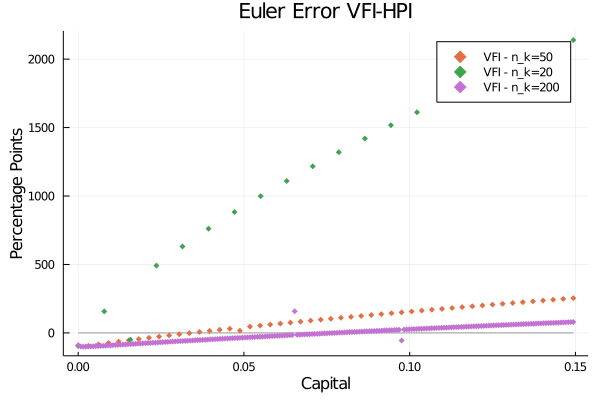
\includegraphics[width=0.65\linewidth]{Assignment2/graphs/HPI_Euler} 

}

\caption{HPI-VFI}\label{fig:unnamed-chunk-3}
\end{figure}

\begin{figure}

{\centering \includegraphics[width=0.65\linewidth]{Assignment2/graphs/MPB_V} \includegraphics[width=0.65\linewidth]{Assignment2/graphs/MPB_Cap} \includegraphics[width=0.65\linewidth]{Assignment2/graphs/MPB_Euler} 

}

\caption{MPB-VFI}\label{fig:unnamed-chunk-4}
\end{figure}

\begin{longtable}[]{@{}llll@{}}
\toprule
Section & ncalls & time & alloc\tabularnewline
\midrule
\endhead
Plain VFI n\_k=200 & 1 & 7209s & 1709GiB\tabularnewline
Plain VFI n\_k=50 & 1 & 464s & 107GiB\tabularnewline
Plain VFI-MPB n\_k=500 & 1 & 236s & 63.3GiB\tabularnewline
Plain VFI-MPB n\_k=200 & 1 & 79.1s & 20.0GiB\tabularnewline
Plain VFI n\_k=20 & 1 & 74.0s & 16.4GiB\tabularnewline
Plain VFI-HPI n\_k=500 & 1 & 59.5s & 15.3GiB\tabularnewline
Plain VFI-MPB n\_k=50 & 1 & 20.2s & 4.27GiB\tabularnewline
Plain VFI-HPI n\_k=200 & 1 & 14.3s & 2.70GiB\tabularnewline
Plain VFI-HPI n\_k=50 & 1 & 3.92s & 261MiB\tabularnewline
Plain VFI-HPI n\_k=20 & 1 & 3.64s & 82.2MiB\tabularnewline
Plain VFI-MPB n\_k=20 & 1 & 182ms & 22.3MiB\tabularnewline
\bottomrule
\end{longtable}

\end{document}
